\documentclass[12pt, twoside]{article}
\input{../preamble}
\usetikzlibrary{calc}

\title{IB}
\author{Chris Huson}
\date{March 2026}

\fancyhead[LE]{\thepage}
\fancyhead[LO]{La Scuola d'Italia / Huson / IB Math: Geometry Review \\* 21 March 2026}

\fancypagestyle{firstpage}{%
  \fancyhf{}%
  \fancyhead[RO]{First \& last name: \hspace{2.25cm} \,\\ \,}%
  \fancyhead[LO]{La Scuola d'Italia / Huson / IB Math: Geometry Review \\* 21 March 2026}%
}

\begin{document}
\thispagestyle{firstpage}

\subsubsection*{9.6 Classwork: Geometry Review (Non-calculator)}

\textit{Formula sheet reference (Topics 3.2--3.3):}
\begin{center}
$\displaystyle \frac{a}{\sin A} = \frac{b}{\sin B} = \frac{c}{\sin C}$
\qquad
$c^2 = a^2 + b^2 - 2ab\cos C$
\qquad
$\text{Area} = \frac{1}{2}ab\sin C$

\vspace{0.3cm}
$l = r\theta$ \qquad $A = \frac{1}{2}r^2\theta$
\end{center}

\vspace{0.1cm}
\textit{Exact values:} $\displaystyle \cos\frac{\pi}{3} = \frac{1}{2}$, \quad $\displaystyle \sin\frac{\pi}{3} = \frac{\sqrt{3}}{2}$

\begin{enumerate}[itemsep=0.5cm]

\item A triangle $OAB$ is inscribed in a circle with centre $O$ and radius $5$. The angle $A\hat{O}B = \dfrac{\pi}{3}$ radians, and $OA = OB = 5$.

\begin{minipage}[t]{0.45\textwidth}
\vspace{0pt}
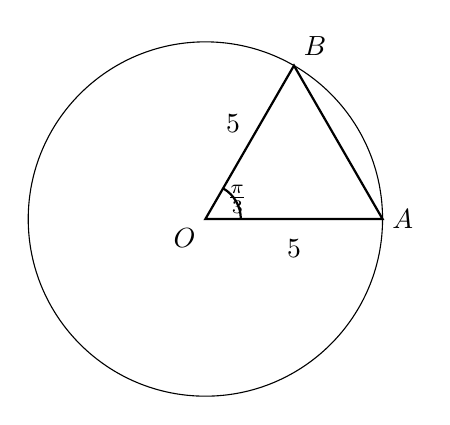
\begin{tikzpicture}[scale=0.45]
    \draw (0,0) circle (5);
    \coordinate (O) at (0,0);
    \coordinate (A) at (0:5);
    \coordinate (B) at (60:5);
    \draw[thick] (O) -- (A) -- (B) -- cycle;
    \draw[thick] (1,0) arc[start angle=0, end angle=60, radius=1];
    \node at (0.9,0.55) {$\frac{\pi}{3}$};
    \node[below left] at (O) {$O$};
    \node[right] at (A) {$A$};
    \node[above right] at (B) {$B$};
    \node[below] at (2.5,-0.3) {$5$};
    \node[above left] at ($(O)!0.5!(B)$) {$5$};
\end{tikzpicture}
\end{minipage}%
\begin{minipage}[t]{0.55\textwidth}
\vspace{0.5cm}
    \begin{enumerate}[itemsep=0.15cm]
        \item Find the length of the arc $AB$. \hfill [2]
        \item Find the area of the sector $OAB$. \hfill [2]
        \item Using the cosine rule, find the length of $AB$. \hfill [3]
        \item Find the area of triangle $OAB$. \hfill [2]
        \item Hence, find the area of the segment (the region between the chord $AB$ and the arc $AB$). \hfill [2]
    \end{enumerate}
\end{minipage}

    \begin{tikzpicture}
        \draw (0,0) rectangle (15.5,10);
        \foreach \y in {1,...,9} \draw [dotted] (0.5,\y)--(15,\y);
    \end{tikzpicture}

\newpage
\item The following diagram shows triangle $PQR$, where $PQ = 8$, $QR = 6$, and $P\hat{Q}R = \dfrac{\pi}{4}$ radians.

\begin{center}
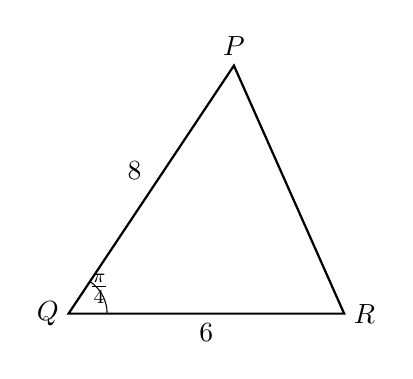
\begin{tikzpicture}[scale=0.7]
    \coordinate (Q) at (0,0);
    \coordinate (P) at (3,4.5);
    \coordinate (R) at (5,0);
    \draw[thick] (Q) -- (P) -- (R) -- cycle;
    \node[left] at (Q) {$Q$};
    \node[above] at (P) {$P$};
    \node[right] at (R) {$R$};
    \node[above left] at ($(Q)!0.5!(P)$) {$8$};
    \node[below] at ($(Q)!0.5!(R)$) {$6$};
    \draw (0.7,0) arc[start angle=0, end angle=56, radius=0.7];
    \node at (0.55,0.45) {$\frac{\pi}{4}$};
\end{tikzpicture}
\end{center}

\textit{Exact values:} $\displaystyle \cos\frac{\pi}{4} = \frac{\sqrt{2}}{2}$, \quad $\displaystyle \sin\frac{\pi}{4} = \frac{\sqrt{2}}{2}$

    \begin{enumerate}[itemsep=0.15cm]
        \item Find the exact area of triangle $PQR$. \hfill [2]
        \item Find the exact length of $PR$. \hfill [3]
        \item Using the sine rule, find $\sin(\hat{R})$. Leave your answer in exact form. \hfill [3]
    \end{enumerate}
    \begin{tikzpicture}
        \draw (0,0) rectangle (15.5,10);
        \foreach \y in {1,...,9} \draw [dotted] (0.5,\y)--(15,\y);
    \end{tikzpicture}

\newpage
\item A circle has centre $O$ and radius $4\,\text{cm}$. Points $P$, $Q$ and $R$ lie on the circumference, and $P\hat{O}R = \theta$ radians. The arc $PQR$ has length $10\,\text{cm}$.

\begin{center}
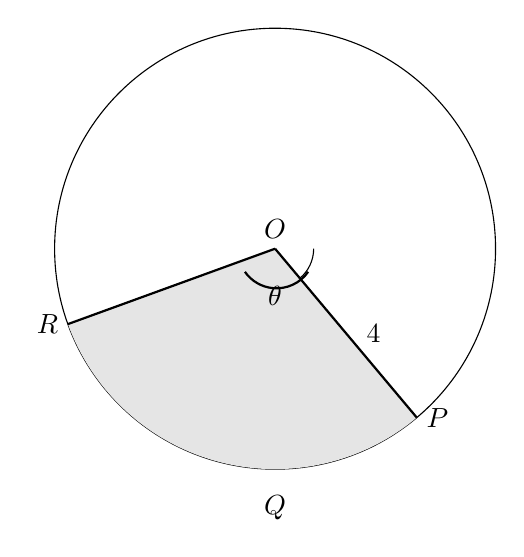
\begin{tikzpicture}[scale=0.7]
    \coordinate (O) at (0,0);
    \coordinate (P) at (-50:4);
    \coordinate (R) at (200:4);
    \draw (0,0) circle (4);
    \fill[gray!20] (O) -- (P) arc[start angle=-50, end angle=-160, radius=4] -- cycle;
    \draw[thick] (O) -- (P);
    \draw[thick] (O) -- (R);
    \draw (0.7,0) arc[start angle=0, end angle=-50, radius=0.7];
    \node[below] at (0,-0.5) {$\theta$};
    \node[right] at (P) {$P$};
    \node[left] at (R) {$R$};
    \node[above] at (O) {$O$};
    \node[below] at (0,-4.3) {$Q$};
    \node[right] at ($(O)!0.5!(P)+(0.2,0)$) {$4$};
    % Draw the angle arc
    \draw[thick] (0.6,-0.42) arc[start angle=-35, end angle=-145, radius=0.7];
\end{tikzpicture}
\end{center}

    \begin{enumerate}[itemsep=0.15cm]
        \item Find the perimeter of the shaded sector. \hfill [2]
        \item Find $\theta$. \hfill [2]
        \item Find the area of the shaded sector. \hfill [2]
    \end{enumerate}

    \hfill \textit{(IB AA SL, 2023 May P1 TZ2, Q1)}
    \begin{tikzpicture}
        \draw (0,0) rectangle (15.5,10);
        \foreach \y in {1,...,9} \draw [dotted] (0.5,\y)--(15,\y);
    \end{tikzpicture}

\newpage
\item The following diagram shows triangle $ABC$, with $AB = 10$, $BC = x$, and $AC = 2x$.

Given that $\cos\hat{C} = \dfrac{3}{4}$, find the area of the triangle.

Give your answer in the form $\dfrac{p\sqrt{q}}{2}$ where $p, q \in \mathbb{Z}^+$. \hfill \textbf{[7]}

    \hfill \textit{(IB AA SL, 2021 May P1 TZ2, Q6)}
    \begin{tikzpicture}
        \draw (0,0) rectangle (15.5,14);
        \foreach \y in {1,...,13} \draw [dotted] (0.5,\y)--(15,\y);
    \end{tikzpicture}

\newpage
\item Consider triangle $ABC$, where $AC = 12$, $CB = 7$, and $B\hat{A}C = 25^\circ$.

Find the smallest possible perimeter of triangle $ABC$. \hfill \textbf{[5]}

    \hfill \textit{(IB AA SL, 2021 Nov P2, Q3) --- calculator allowed}
    \begin{tikzpicture}
        \draw (0,0) rectangle (15.5,14);
        \foreach \y in {1,...,13} \draw [dotted] (0.5,\y)--(15,\y);
    \end{tikzpicture}

\newpage
\item The cities Lucknow ($L$), Jaipur ($J$), and Delhi ($D$) are represented in the following diagram. Lucknow lies 500\,km directly east of Jaipur, and $J\hat{L}D = 25^\circ$. The bearing of $D$ from $J$ is $034^\circ$.

    \begin{enumerate}[itemsep=0.15cm]
        \item Find $J\hat{D}L$. \hfill [2]
        \item Find the distance between Lucknow and Delhi. \hfill [3]
    \end{enumerate}

    \hfill \textit{(IB AA SL, 2023 May P2 TZ1, Q1) --- calculator allowed}
    \begin{tikzpicture}
        \draw (0,0) rectangle (15.5,11);
        \foreach \y in {1,...,10} \draw [dotted] (0.5,\y)--(15,\y);
    \end{tikzpicture}

\newpage
\item A farmer is placing posts at points $A$, $B$, and $C$ in the ground to mark the boundaries of a triangular piece of land on his property.

From point $A$, he walks due west 230 metres to point $B$. From point $B$, he walks 175 metres on a bearing of $063^\circ$ to reach point $C$.

    \begin{enumerate}[itemsep=0.15cm]
        \item Find the distance from point $A$ to point $C$. \hfill [4]
        \item Find the area of this piece of land. \hfill [2]
        \item Find $C\hat{A}B$. \hfill [3]
        \item The farmer wants to divide the piece of land into two sections. He will put a post at point $D$, which is between $A$ and $C$. He wants the boundary $BD$ to divide the piece of land such that the sections have equal area. Find the distance from point $B$ to point $D$. \hfill [5]
    \end{enumerate}

    \hfill \textit{(IB AA SL, 2023 May P2 TZ2, Q7) --- calculator allowed}
    \begin{tikzpicture}
        \draw (0,0) rectangle (15.5,9);
        \foreach \y in {1,...,8} \draw [dotted] (0.5,\y)--(15,\y);
    \end{tikzpicture}

\end{enumerate}
\end{document}
Solutions
  Problem 1 — Circle with radius 5, angle π/3:
  - (a) l = rθ = 5 × π/3 = 5π/3
  - (b) A = ½r²θ = ½(25)(π/3) = 25π/6
  - (c) c² = 5² + 5² − 2(5)(5)cos(π/3) = 25 + 25 − 50(½) = 25, so AB = 5
      (Triangle OAB is equilateral)
  - (d) Area = ½(5)(5)sin(π/3) = 25√3/4
  - (e) Segment = sector − triangle = 25π/6 − 25√3/4

  Problem 2 — Triangle PQR with sides 8, 6 and angle π/4:
  - (a) Area = ½(8)(6)sin(π/4) = 24 × √2/2 = 12√2
  - (b) PR² = 8² + 6² − 2(8)(6)cos(π/4) = 64 + 36 − 96(√2/2) = 100 − 48√2
      PR = √(100 − 48√2)
  - (c) By sine rule: sin(R)/8 = sin(π/4)/PR
      sin(R) = 8sin(π/4)/√(100 − 48√2) = 4√2/√(100 − 48√2)

  Problem 3 — Circle radius 4, arc length 10:
  - (a) Perimeter = arc + 2r = 10 + 8 = 18 cm
  - (b) l = rθ → 10 = 4θ → θ = 5/2 = 2.5 radians
  - (c) A = ½r²θ = ½(16)(5/2) = 20 cm²

  Problem 4 — Cosine rule with cos C = 3/4, sides x, 2x, 10:
  - By cosine rule: 10² = x² + (2x)² − 2(x)(2x)(3/4)
    100 = x² + 4x² − 3x² = 2x², so x² = 50, x = 5√2
  - sin C: sin²C + cos²C = 1 → sin²C = 1 − 9/16 = 7/16 → sin C = √7/4
  - Area = ½(x)(2x)sin C = ½(5√2)(10√2)(√7/4) = ½(100)(√7/4) = 25√7/2

  Problem 5 — Ambiguous case: AC=12, CB=7, angle A=25°:
  - Sine rule: sin C/12 = sin 25°/7
    sin C = 12 sin 25°/7 ≈ 0.7240
    C₁ ≈ 46.4° or C₂ ≈ 133.6°
  - B₁ = 180 − 25 − 46.4 = 108.6°, B₂ = 180 − 25 − 133.6 = 21.4°
  - AB₁ = 7 sin 108.6°/sin 25° ≈ 15.7, AB₂ = 7 sin 21.4°/sin 25° ≈ 6.04
  - Perimeter₁ ≈ 34.7, Perimeter₂ ≈ 25.0
  - Smallest perimeter ≈ 25.0

  Problem 6 — Bearings: Lucknow-Jaipur-Delhi:
  - Angle DJL: bearing 034° from north, JL is due east (090°), so DJL = 90 − 34 = 56°
  - Angle sum: JDL = 180 − 56 − 25 = 99°
  - Sine rule: DL/sin 56° = 500/sin 99° → DL = 500 sin 56°/sin 99° ≈ 420 km

  Problem 7 — Farmer's land:
  - (a) BA is due east. Bearing of C from B is 063°. Angle ABC = 090° − 063° = 27°.
    AC² = 230² + 175² − 2(230)(175)cos 27° ≈ 11803, AC ≈ 108.6 m
  - (b) Area = ½(230)(175)sin 27° ≈ 9137 m²
  - (c) sin(CAB)/175 = sin 27°/AC → CAB ≈ 47.2°
  - (d) Equal areas → AD = AC/2. Use cosine rule in triangle ABD to find BD.
